\documentclass[11pt, letterpaper, onecolumn]{exam}

% 定义作业名
\newcommand{\Homework}{操作系统第五次作业}

% 定义姓名、学号和班级的命令
\newcommand{\Name}{蓝宇舟}
\newcommand{\StudentNumber}{2022K8009918005}
\newcommand{\Class}{计算机科学与技术}

\usepackage[a4paper]{geometry}
\geometry{left=2.0cm,right=2.0cm,top=2.5cm,bottom=2.5cm}

\usepackage[scheme=plain]{ctex} % 支持中文的LaTeX宏包
\usepackage{float} % 防止图片乱序
\usepackage{xeCJK} % 中文字体
\usepackage{fontspec} % 字体设置
\usepackage{lastpage} % 获取总页数
\usepackage{amsmath,amsfonts,graphicx,subfigure,amssymb,bm,amsthm,mathrsfs,
mathtools,breqn} % 数学公式和符号的宏包集合
\usepackage{algorithm,algorithmicx} % 算法和伪代码
\usepackage[noend]{algpseudocode} % 算法和伪代码
\usepackage[framemethod=TikZ]{mdframed} % 创建带边框的框架
\usepackage{adjustbox} % 调整盒子大小
\usepackage{fontsize} % 设置字体大小
\usepackage{tikz,xcolor} % 绘制图形和使用颜色
\usepackage{multicol} % 多栏排版
\usepackage{multirow} % 表格中合并单元格
\usepackage{pdfpages} % 插入PDF文件
\usepackage{listings} % 在文档中插入源代码
\usepackage{lstautogobble} % 去掉源代码多余的空格
\usepackage{xcolor} % 支持彩色
\usepackage{caption} % 支持图片标题
\usepackage{wrapfig} % 文字绕排图片
\usepackage{bigstrut,multirow,rotating} % 支持在表格中使用特殊命令
\usepackage{booktabs} % 创建美观的表格
\usepackage{circuitikz} % 绘制电路图
\usepackage{zhnumber} % 中文序号(用于标题)
\usepackage{tabularx} % 表格折行
\usepackage{enumitem} % 枚举列表
\usepackage{xparse} % 支持更多的命令定义
% \usepackage{fancyhdr} % 页眉页脚
\usetikzlibrary{circuits.ee.IEC} % 使用欧洲风格的电路符号
\usetikzlibrary{circuits.logic.US} % 使用美国风格的逻辑门
\usetikzlibrary{shapes.geometric, arrows.meta, positioning} % 使用流程图的库

\usepackage{hyperref} % 目录,章节,超链接
\hypersetup{
    bookmarks=true,  % 生成书签
    bookmarksnumbered=true  % 书签带章节编号
}

% 轻松引用, 可以用\cref{}指令直接引用, 自动加前缀.
% 例: 图片label为fig:1
% \cref{fig:1} => Figure.1
% \ref{fig:1}  => 1
\usepackage[capitalize]{cleveref}
% \crefname{section}{Sec.}{Secs.}
\Crefname{section}{Section}{Sections}
\Crefname{table}{Table}{Tables}
\crefname{table}{Table.}{Tabs.}

\section{环境说明}

\begin{itemize}
    \item 操作系统:{\tt Arch Linux x86_64}
    \item 内核版本:{\tt Linux 6.10.7-zen1-1-zen}
    \item 编译器版本:{\tt gcc (GCC) 14.2.1 20240805}
\end{itemize}


\begin{document}

% 标题
\begingroup
    \centering
    \LARGE {\bf \Homework} \\[0.5em]
    \large \textbf{姓名:} \Name \hspace{2em}
           \textbf{学号:} \StudentNumber \hspace{2em}
           \textbf{班级:} \Class \par
\endgroup
\rule{\textwidth}{0.4pt}
\printanswers


% 环境
\section{环境说明}

\begin{itemize}
    \item 操作系统:{\tt Arch Linux x86_64}
    \item 内核版本:{\tt Linux 6.10.7-zen1-1-zen}
    \item 编译器版本:{\tt gcc (GCC) 14.2.1 20240805}
\end{itemize}


% 正文
\section{作业正文}

\begin{questions}

\question {
    现有一个由$5$块磁盘组成的磁盘阵列,采用 RAID-5 模式,如下图所示。
}

\begin{figure}[H]
    \centering
    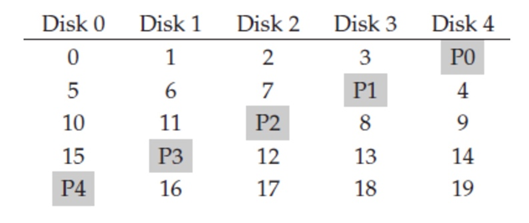
\includegraphics[width=0.6\textwidth]{img/q1.png}
\end{figure}

该磁盘阵列每个硬盘的块(block)大小为 4KB,每条(strip)含一个块;磁盘的平均寻道时间是 4ms,
旋转速度是 7200 RPM (每分钟 7200 转),传输带宽是 200MB/s,请计算:

\begin{parts}
    \part {
        平均来说,从该 RAID5 阵列上读出一个条带(stripe)的时间是多少?
    }
    \part {
        当向该 RAID5 阵列中写入连续的两个 4KB 数据块时,平均来说,所需的时间是多少?
        请考虑这两个数据块属于同一个条带和不同条带的两种情况。
    }
\end{parts}

\begin{solution}

\begin{parts}

\part

平均寻道时间为
$$
    T_{seek} = 4 \text{ms}
$$

平均旋转时间为
$$
    T_{rotation} = \frac{1}{2}(60/7200)  \approx 4.17 \text{ms}
$$

平均传输时间为
$$
    T_{transfer} = 4 \text{KB} / 200 \text{MB} = 0.02 \text{ms}
$$

因为读取一个条带,五个磁盘可以并行读取,所以总时间就是单个磁盘读取一个块的时间:
$$
    T = T_{seek} + T_{rotation} + T_{transfer} = 8.19 \text{ms}
$$

\part

写操作流程如下:

\begin{enumerate}
    \item 读旧块
    \item 读旧校验块
    \item 计算新校验块: $P_{new} = (B_{old} \oplus B_{new}) \oplus P{old}$
    \item 写新块
    \item 写新校验块
\end{enumerate}

包含 4 次磁盘访问。

对于两个数据属于同一条带的情况,两个数据块和其校验块在同一个条带,1、2 和 4、5 步可以分别同时进行。
计算时间可以忽略不计。所以共需要 2 次磁盘访问。

所需时间为:

$$
    T_1 = T \times 2 = 16.38 \text{ms}
$$

对于两个数据属于不同条带的情况,每个数据块和其校验块在同一个条带,1、2 和 4、5 步可以分别同时进行。
计算时间可以忽略不计。所以共需要 4 次磁盘访问。

所需时间为:

$$
    T_1 = T \times 4 = 32.76 \text{ms}
$$

\end{parts}

\end{solution}

\question {
    假设一台计算机使用 32-bit 的虚拟地址空间和三级页表,虚地址的划分为 8-bit | 6-bit | 6-bit | 12-bit(注:8 bit 对应为第一级页表的地址,以此类推),请计算:
}

\begin{parts}
    \part 该计算机系统的页大小是多少?
    \part 该三级页表一共能索引多少个页?
    \part 现有一个程序的代码段大小为 128KB,数据段为 66KB,栈大小为 8KB,则在使用上述三级
    页表时,最少需要占用多少个物理页框?最多会占用多少个物理页框?(注:假设程序各段在地址空间
    中的布局可以自行决定)
    \part 假设该计算机使用一级页表进行地址空间管理,则上一问中程序需要占用多少个物理页框?
\end{parts}


\begin{solution}

\begin{parts}

\part
页大小为
$$
    2^{12} = 4096 \text{ B} = 4 \text{ KB}
$$

\part
三级页表一共能索引的页数为
$$
    2^{8+6+6} = 2^{20} \text{ Pages} = 1 \text{ M Pages}
$$

\part {
    最少情况:代码段、数据段和栈分别占据$31$、$17$和$2$页,即共占据$51$页,最少需要占用$51$个物理
    页框,少于一级页表能索引的页数$2^6=64$。因此可以放在同一个一级页表内。所以最少需要的物理页框数
    为$1$个三级页表,$1$个二级页表,$1$个一级页表,以及虚拟页本身的$51$个物理页框,共$54$个物理页框。

    最多情况:代码段、数据段和栈在虚拟地址空间分散排布,由于这三者最少需要两页,所以对于其中任何一个,
    都可以跨越一级页表和二级页表。因此最多需要的物理页框数为$1$个三级页表,$2 \times 3 = 6$个二级
    页表,$2 \times 3 = 6$个一级页表,以及虚拟页本身的$51$个物理页框,共$64$个物理页框。
}

\part
如果使用一级页表进行地址空间管理,则只需要$1$个一级页表和虚拟页本身的$51$个物理页框,共$52$个物理页框。

\end{parts}

\end{solution}


\end{questions}


\end{document}
